\documentclass[aspectratio=1610,12pt]{beamer}

\usepackage{tikz}
\usetikzlibrary{calc}
\usetikzlibrary{graphs}
\usetikzlibrary{cd}
\usetikzlibrary{patterns}
\usetikzlibrary{backgrounds}
\usetikzlibrary{shapes}
\usetikzlibrary{decorations.pathmorphing}
\usetikzlibrary{decorations.pathreplacing}
%\usepackage{libertine}
\usepackage{stmaryrd}
\usepackage{tikz-cd}
\usepackage{ebproof}
\usepackage{minted}
\usepackage{booktabs}
%\usepackage{colortbl}

% Definitions {{{

% ACM palette {{{
\definecolor[named]{ACMBlue}{cmyk}{1,0.1,0,0.1}
\definecolor[named]{ACMYellow}{cmyk}{0,0.16,1,0}
\definecolor[named]{ACMOrange}{cmyk}{0,0.42,1,0.01}
\definecolor[named]{ACMRed}{cmyk}{0,0.90,0.86,0}
\definecolor[named]{ACMLightBlue}{cmyk}{0.49,0.01,0,0}
\definecolor[named]{ACMGreen}{cmyk}{0.20,0,1,0.19}
\definecolor[named]{ACMPurple}{cmyk}{0.55,1,0,0.15}
\definecolor[named]{ACMDarkBlue}{cmyk}{1,0.58,0,0.21}
% }}}

% Parameters {{{
\newcommand{\figsize}{\small}
\usecolortheme[named=ACMDarkBlue]{structure}

\addtobeamertemplate{navigation symbols}{}{%
    \usebeamerfont{footline}%
    \usebeamercolor[fg]{footline}%
    \hspace{1em}%
    \insertframenumber/\inserttotalframenumber
}

\AtBeginSection[] % Do nothing for \section*
{
\begin{frame}<beamer>
\frametitle{Outline}
\tableofcontents[currentsection]
\end{frame}
}

%}}}

% String diagrams {{{
\colorlet{sdbg}{lightgray!50!white}
\colorlet{scsdbg}{lightgray!50!white}
\colorlet{tssdbg}{lightgray!50!white}
\colorlet{memsdbg}{ACMLightBlue!50!white}
\colorlet{mmemsdbg}{ACMBlue!50!white}
\colorlet{penvsdbg}{ACMGreen!50!white}

% String diagram picture
\tikzset{sdp/.style={
  x=4mm,
  y=3.5mm,
  z={(1.6mm,1.6mm)}
}}
% String diagram node
\tikzset{sdn/.style={
  draw,
  fill=white,
  shape=rectangle,
  rounded corners,
}}
% Nodes for terminator
\tikzset{bln/.style={
  sdn,
  shape=circle,
  inner sep=1pt,
}}
% Nodes for 3d transition systems
\tikzset{tst/.style={xslant=1,yscale=0.7}}
\tikzset{tsn/.style={sdn,tst}}
% Nodes for 3d simulation conventions
\tikzset{sct/.style={yslant=1,xscale=0.7,yscale=1.2}}
\tikzset{scn/.style={sdn,inner sep=2pt,sct}}
% Active region
\tikzset{act/.style={
  pattern=north west lines,
  opacity=0.33
}}

\newcommand{\companion}{
  node[sct] {\tikz\draw[-Stealth] (0,0);}
}
\newcommand{\conjoint}{
  node[sct,rotate=180] {\tikz\draw[-Stealth] (0,0);}
}

\newcommand{\flatcompanion}{
  node {\tikz\draw[-Stealth] (0,0);}
}
\newcommand{\flatconjoint}{
  node[rotate=180] {\tikz\draw[-Stealth] (0,0);}
}

% }}}

\newcommand\lensarrow\leftrightarrows
\newcommand\lensle\equiv

% Macros {{{

% Some of the macros I defined trip up latexdiff,
% so I separate them in this file.
% vim: foldmethod=marker

% Notations
\newcommand{\kw}[1]{\ensuremath{ \mathsf{#1} }}
\newcommand{\ifr}[1]{\mathrel{[{#1}]}}
\newcommand{\que}{\circ}
\newcommand{\ans}{\bullet}
\newcommand{\vref}{\le_\kw{v}}
\newcommand{\mext}{\le_\kw{m}}
\newcommand{\refby}{\preceq}
\newcommand{\scref}{\sqsupseteq}
\newcommand{\screfd}{\sqsubseteq}
\newcommand{\unitset}{\mathds{1}}

% Multi-letter language interfaces
\newcommand{\li}[1]{\mathit{#1}}
% Calling conventions (language interface boundaries)
\newcommand{\cc}[2]{{ \kw{#1#2} }}

% Pointers for justified sequences %{{{

% Parameters
\newcommand{\pshift}{1.6ex}
\newcommand{\pcdist}{1}
\newcommand{\pcangle}{60}

% Pointer hook
\newcommand{\ph}[1]{%
  \tikz[remember picture]{\coordinate (#1);}}

% Pointer to
\newcommand{\ptc}[2]{%
  \tikz[remember picture,baseline,>={Latex[round,length=3.6pt]}]{
    \draw[->,#2]
      let \p{dest} = (#1),
          \n1 = {pow(veclen(\x{dest}, \y{dest}), 0.5) * 1.5},
          \p1 = ($(0,0)+(0,\pshift)$),
          \p4 = ($(\x{dest},0)+(0,\pshift)$),
          \p2 = ($(\p1)!\n1*\pcdist!-\pcangle:(\p4)$),
          \p3 = ($(\p4)!\n1*\pcdist!+\pcangle:(\p1)$) in
        (\p1) .. controls (\p2) and (\p3) .. node[pos=0.5] (top) {} (\p4);
    \pgfresetboundingbox
    \path[use as bounding box] (0,0 |- top);
}}
\newcommand{\pt}[1]{%
  \ptc{#1}{gray}}
\newcommand{\bpt}[1]{%
  \ptc{#1}{black,thick,>={Latex[round,length=4pt]}}}

% TikZ setup
\pgfdeclarelayer{tint}
\pgfdeclarelayer{nodes}
\pgfsetlayers{tint,background,main,nodes}
\selectcolormodel{cmyk}

% Parameters for diagrams
\newcommand{\stens}{0.6}

% The intensity of colors in figures and row highlighting respectively.
% These should be the same, otherwise they are just confusing to look at
% side by side, especially on a printout.
\newcommand{\filltint}{!35}
\newcommand{\tbltint}{\filltint}

% Colors used in the World transitions section
\newcommand{\colorA}{ACMDarkBlue}
\newcommand{\colorB}{ACMDarkBlue}
\newcommand{\internalA}[1]{\textcolor{\colorA}{#1}}
\newcommand{\internalB}[1]{\textcolor{\colorB}{#1}}

% Refinement tiles {{{

\newenvironment{tile}[1]{%
  \begin{tikzpicture}[baseline,yscale=0.36,xscale=0.5]
    \figsize
    \tikzset{to path={
      .. controls ($(\tikztostart)!\stens!(\tikztostart -| \tikztotarget)$)
              and ($(\tikztotarget)!\stens!(\tikztotarget -| \tikztostart)$) ..
      (\tikztotarget) \tikztonodes}}
    \tikzset{#1}
    % Coordinates for things on the left
    \coordinate (TL) at (-1,1);
    \coordinate (L) at (-1,0);
    \coordinate (BL) at (-1,-1);
    \coordinate (TLB) at (-0.3,1);
    \coordinate (BLB) at (-0.3,-1);
    % Coordinates for things on the right
    \coordinate (TR) at (1,1);
    \coordinate (R) at (1,0);
    \coordinate (BR) at (1,-1);
    \coordinate (TRB) at (0.3,1);
    \coordinate (BRB) at (0.3,-1);
    % Center node, for crossing
    \coordinate (T) at (0,+1.5);
    \node[circle,inner sep=2pt] (C) at (0,0) {};
    \coordinate (B) at (0,-1.5);
    % Computed coordinates
    \coordinate (TLC) at ($(T-|L)$);
    \coordinate (BLC) at ($(B-|L)$);
    \coordinate (TRC) at ($(T-|R)$);
    \coordinate (BRC) at ($(B-|R)$);
}{%
  \end{tikzpicture}
}
\newcommand{\simproof}[2]{%
  \begin{pgfonlayer}{nodes}
    \node[draw,rectangle,fill=white,rounded corners=2pt,minimum height=0.5cm,minimum width=0.8cm] at #1 {#2};
  \end{pgfonlayer}
}
\newcommand{\drawsc}{%
  \draw[thick,rounded corners=1mm]
}
\newcommand{\filltop}[1]{%
  \begin{pgfonlayer}{tint}
    \fill[#1] (TLC) rectangle (R);
  \end{pgfonlayer}
}
\newcommand{\fillbot}[1]{%
  \begin{pgfonlayer}{tint}
    \fill[#1] (L) rectangle (BRC);
  \end{pgfonlayer}
}
\newcommand{\fillboth}[1]}}



%\renewcommand{\filltint}{!40}

\newcommand{\drawsb}[2]{%
  \draw (#1) -- node[pos=0.6] (sbT) {} +(-0.2ex,0) |- (#1 |- #2);
  \draw (sbT.center) -- (sbT.center |- #2);
  \draw (#1 -| #2) -- node[pos=0.6] (sbT) {} +(0.2ex,0) |- (#2);
  \draw (sbT.center) -- (sbT.center |- #2);
}

\newcommand{\cprog}[2]{
  \begin{scope}[every node/.style={align=left,inner sep=1ex}]
    \scriptsize \tt
    \node<#1> (C1) at (0,2) {
      int mult(n, p) \{ \\
      \:\: return n * p; \\
      \}
    };
    \node<#2> (C2) at (1,2) {
      int sqr(n) \{ \\
      \:\: return mult(n, n); \\
      \}
    };
    \node<#1> (C3) at (2,2) {
      int main() \{ \\
      \:\: return sqr(3); \\
      \}
    };
  \end{scope}
}

\newcommand{\sprog}[3]{
  \begin{scope}[every node/.style={align=left,inner sep=1ex}]
    \scriptsize \tt
    \setlength{\tabcolsep}{0.5ex}
    \node<#1> (#31) at (0,#2) {
      \begin{tabular}{rl}
        mult: & \%eax := \%ebx \\
              & \%eax *= \%ecx \\
              & ret
      \end{tabular}
    };
    \node<#1> (#32) at (1,#2) {
      \begin{tabular}{rl}
        sqr: & \%ecx := \%ebx \\
             & call mult \\
         L1: & ret
      \end{tabular}
    };
    \node<#1> (#33) at (2,#2) {
      \begin{tabular}{rl}
        main: & \%ebx := 3 \\
              & call sqr \\
          L2: & ret
      \end{tabular}
    };
  \end{scope}
}

% }}}

% TikZ pic's {{{

\tikzset{filesys/.pic={
  \begin{scope}[xscale=0.33,yscale=0.5,yshift=0.5cm]
    \tiny
    \node[draw,circle] {\tt /}
      child {node {\tt bin}}
      child {node {\tt etc}}
      child[missing] { }
      child {node {\ldots}};
  \end{scope}
}}
\tikzset{hdd/.pic={
  \begin{scope}[xscale=0.75,yscale=0.25,yshift=-0.66cm]
    \draw[fill,shade,shading angle=90,left color=ACMGreen,right color=ACMGreen\filltint]
      (-1,1) arc[start angle=-180,end angle=0,radius=1] --
      (+1,0) arc[start angle=0,end angle=-180,radius=1] --
      cycle;
    \draw[fill=ACMGreen] (0,1) ellipse[radius=1];
    \draw (-1,0.33) arc[start angle=-180,end angle=0,radius=1];
    \draw (-1,0.66) arc[start angle=-180,end angle=0,radius=1];
  \end{scope}
}}

\tikzset{cpu/.pic={
  \begin{scope}[scale=0.4]
    \tikzset{every path/.style={
      decoration={
        border,
        angle=-90,
        segment length=1mm,
        amplitude=2mm,
        pre=moveto,
        pre length=2mm,
        %post=moveto,
        %post length=0.5mm
      }
    }}
    \draw[fill=ACMRed\filltint] (-1,-1) rectangle (+1,+1);
    \node {\scriptsize CPU};
    \draw[decorate] (-1,-1) -- (+1,-1);
    \draw[decorate] (+1,-1) -- (+1,+1);
    \draw[decorate] (+1,+1) -- (-1,+1);
    \draw[decorate] (-1,+1) -- (-1,-1);
    %\draw (+1,-1) -- (+1,+1);
     % -- (-1,+1) -- cycle;
  \end{scope}
}}

\tikzset{nic/.pic={
  \begin{scope}[xscale=0.15,yscale=0.2,xshift=-3.5cm,yshift=-2.5cm]
    \draw[fill=ACMGreen] (7,4) -| (0,1) -| (1,0) -| (4,1) -| (5,0) -| (6,1) -- (7,1);
    \draw[thick] (7,0) |- (8,5);
    \node at (3.5,2.5) {\scriptsize NIC};
    \tikzset{every path/.style={
      ACMYellow,
      thick,
      decoration={
        border,
        angle=90,
        segment length=0.5mm,
        amplitude=1.8mm
      }
    }}
    \draw[decorate] (1.33,0.1) -- (4,0.1);
    \draw[decorate] (5.33,0.1) -- (6,0.1);
  \end{scope}
}}

\tikzset{eth/.pic={
  \begin{scope}[scale=0.2,xscale=1.5,yshift=-5mm,xshift=-2cm]
    \draw[fill=ACMYellow\filltint]
      (0,0) rectangle (1,1);
    \draw[ACMYellow!80!black,decorate,decoration={
        border,angle=-90,segment length=0.25mm,amplitude=1.5mm}]
      (0.05,0.18) -- (0.05,1);
    \fill[ACMYellow] (1,2.5mm) rectangle (5,7.5mm);
    \draw (5,2.5mm) -- (1,2.5mm) (1,7.5mm) -- (5,7.5mm) -- cycle;
  \end{scope}
}}

%}}}

%}}}

% Front matter {{{
\title{Three Dimensions of Compositionality
  in~CompCert~Semantics}
\author{Jérémie Koenig}
\institute{Yale University}
%\date{PLDI '21, June 20--25, 2021}
%\date{Yale CSL, April 30, 2021}
\date{MFPS, June 21, 2023}
\titlegraphic{
  \begin{tile}{xscale=1.5}
    \simproof{(C)}{$\le$}
    \draw[thick] (L) -- (R);
    \draw (T) -- (B);
    \begin{pgfonlayer}{tint}
      \fill[ACMLightBlue\filltint] (TLC) rectangle (C.center);
      \fill[ACMOrange\filltint] (L) rectangle (B);
      \fill[ACMBlue\filltint] (T) rectangle (R);
      \fill[ACMRed\filltint] (C.center) rectangle (BRC);
    \end{pgfonlayer}
  \end{tile}
}
%}}}

\setlength\parskip{1ex}

\begin{document}

\maketitle

\section*{Introduction}

\begin{frame}{Why Compilers are Interesting} %{{{
One notion of compiler correctness is \emph{semantics preservation}:
\[
  \kw{Compile}(p) = p' \quad\Longrightarrow\quad
  \kw{S}\llbracket p \rrbracket \:\le\: \kw{T}\llbracket p' \rrbracket
\]
\pause
In principle,
we can get \emph{compositional} compiler correctness \\
by making $\kw{S}\llbracket - \rrbracket$ and $\kw{T}\llbracket - \rrbracket$
compositional semantics.

\vfill
\pause
But in practice this is hard to do!
\begin{itemize}
\item
$\kw{S}$ and $\kw{T}$
must be interpreted in the same domain
\item
We must formalize the \textbf{calling convention}
\end{itemize}
Traditional compositional semantics
do not deal with that.
\end{frame}
%}}}

\begin{frame}{End-to-end verification of heterogeneous systems} %{{{

  \centering
  \begin{tikzpicture}[xscale=3,yscale=1.8]
    % Set a draw color to use as guide
    % When invisible, it ensures the bounding box is fixed
    \path (-0.5,-0.5) grid (2.5,2.5);

    % We use the following style to introduce invisible nodes to give
    % pictures a "shape" we can use to anchor edges
    \tikzset{blob/.style={
      ellipse,
      %fill=lightgray,
      minimum height=1cm,
      minimum width=1.8cm,
      outer sep=1ex,
    }}

    % For programs, we use text labels with a "C" blue background
    \tikzset{cprog/.style={
      draw,
      fill=ACMLightBlue\filltint,
      rounded corners,
      minimum height=1.6em,
      outer sep=1ex,
    }}

    % 1. We will consider what it means to have a certified web server
    \node[cprog] (WEB) at (1,2) {Web server};

    % 2. A good specification really must model the network and file system
    \only<2->{
      \node[blob] (FS) at (0,2) {}; \pic at (FS.center) {filesys};
      \node[blob] (NET) [cloud,aspect=2,draw,fill=lightgray,inner sep=0.5mm]
        at (2,2) {\scriptsize Network};
      \draw[<->] (FS) -- (WEB);
      \draw[<->] (WEB) -- (NET);
    }

    % 3. But those things are really abstractions, to really verify
    % things we must model the system that actually runs
    \only<3->{
      \node[blob] (HDD) at (0,0) {}; \pic<2-> at (HDD.center) {hdd};
      \node[blob] (CPU) at (1,0) {}; \pic<2-> at (CPU.center) {cpu};
      \node[blob] (NIC) at (2,0) {}; \pic<2-> at (NIC.center) {nic};
      %\node[blob] (ETH) at (3,0) {}; \pic at (ETH.center) {eth};
      \draw[<->] (HDD) -- (CPU);
      \draw[<->] (CPU) -- (NIC);
    }

    % 4. A key question is the relationship between the two
    \only<4->{
      \draw[double equal sign distance,Implies-Implies] (FS) -- (HDD);
      \draw[double equal sign distance,Implies-Implies] (WEB) -- (CPU);
      \draw[double equal sign distance,Implies-Implies] (NET) -- (NIC);
    }

    % 5. In-between, there is a lot of code involved
    \node<5-6>[align=center,fill=white,ellipse] (OS) at (1,1.05)
      {Operating system, \\ compilers, etc.};
    % We do operating systems and compilers, among other things
    \node<7-8> at (1,1.05) {\includegraphics[scale=0.2]{flint-banner}};

    % Thankfully, many of these things have been verified
    \tikzset{checkmark/.style={
      text=ACMGreen,
      node contents=\checkmark,
      overlay,
    }}
    \path<6-7>
      (FS.north east) node[checkmark]
      (WEB.north east) node[checkmark]
      (NET.east) node[right,checkmark]
      (CPU.south east) node[checkmark]
      (OS.north east) node[checkmark];

    % What we need is a glue
    \begin{pgfonlayer}{background}
      \node<9->[overlay,
          ellipse,
          cloud puffs=16,
          minimum height=7cm,
          minimum width=10cm,
          fill=gray!5]
        (GLUE) at (1,1) {};
      \node<9->[overlay,text=ACMGreen] at (GLUE.east) {\Huge \checkmark};
    \end{pgfonlayer}

    \node<8>[ellipse,fill=gray!5,align=center] at (1,1.05)
      {\scriptsize This talk: \\ \Large CompCertO, CAL};

  \end{tikzpicture}
\end{frame}
%}}}

\section{Compositional Semantics in CompCert}

\begin{frame}{Semantics in CompCert} %{{{
  For each source, target and intermediate (whole) program $p \in L$, \\
  a transition system
  $L[p] = \langle S, {\rightarrow}, I, F \rangle$ is defined where:
  \[
    S \in \mathbf{Set} \qquad
    {\rightarrow} \subseteq S \times S \qquad
    I \subseteq S \qquad
    F \subseteq S \times \mathsf{int}
  \]
  \pause
  An execution of $p$ corresponds to a transition sequence:
  \[
    I \ni s_0 \rightarrow s_1 \rightarrow \cdots \rightarrow s_n \mathrel{F} x
  \]

  \pause
  CompCert's correctness is then established as a simulation property:
  \[
    \mathsf{CompCert}(p) = p' \quad\Longrightarrow\quad
    \mathsf{Clight}[p] \:\le\: \mathsf{Asm}[p'] %\:\in\: \mathsf{TS}
    \,,
  \]
  obtained by composing similar
  statements for each compilation pass.
\end{frame}
%}}}

\begin{frame}[fragile]{Simulations} %{{{
  %CompCert is broken down in compilation phases
  %which are verified individually.

  %\vfill
  A simulation $\rho : L_1 \le L_2 \in \mathsf{TS}$ of $L_1$ by $L_2$
  is a relation $\rho \subseteq S_1 \times S_2$ such that:
  \vspace{-1ex}
  \begin{columns}
    \begin{column}{.68\textwidth}
      \begin{itemize}
        \item $s_1 \in I_1 \:\Rightarrow\: \exists s_2 \mathbin.
          s_2 \in I_2 \:\wedge\: s_1 \mathrel{\rho} s_2$
        \item $s_1 \mathrel{\rho} s_2 \:\wedge\: s_1 \rightarrow_1 s_1'
          \:\Rightarrow\: \exists s_2' \mathbin.
            s_2 \rightarrow_2 s_2' \:\wedge\: s_1' \mathrel{\rho} s_2'$
        \item $s_1 \mathrel{\rho} s_2 \:\wedge\: s_1 \mathrel{F_1} x
          \:\Rightarrow\: s_2 \mathrel{F_2} x$,
      \end{itemize}
    \end{column}
    \begin{column}{.25\textwidth}
      \[
      \begin{tikzcd}
        s_1 \ar[d,"\rho"',dash] \ar[r] & s_1' \ar[d,dashed,dash,"\rho"] \\
        s_2 \ar[r,dashed] & s_2'
      \end{tikzcd}
      \]
    \end{column}
  \end{columns}
  \vspace{1ex}
  so that any execution of $L_1$ yields a
  a similar execution of $L_2$.

  \pause
  \begin{columns}
    \begin{column}{.68\textwidth}
  Simulation relations compose in the expected way:
  \[
    \begin{prooftree}
      \hypo{\rho : L_1 \le L_2}
      \hypo{\pi : L_2 \le L_3}
      \infer2{(\rho \mathbin; \pi) : L_1 \le L_3}
    \end{prooftree}
  \]
  making it possible to decompose the correctness proof.
    \end{column}
    \pause
    \begin{column}{.25\textwidth}
      \[
        \begin{tikzcd}[column sep=0.5ex]
          L_1 \ar[d, Rightarrow, "\rho"] &&
          L_1 \ar[dd, Rightarrow, "\rho \mathbin; \pi"] \\
          L_2 \ar[d, Rightarrow, "\pi"] & \vdash \\
          L_3 && L_3
        \end{tikzcd}
      \]
    \end{column}
  \end{columns}
\end{frame}
%}}}

\begin{frame}{Vertical Composition \fbox{$;$}} %{{{
  In other words, transition systems and simulations form a category:
  \begin{itemize}
    \item the objects are transition systems
    \item the morphisms from $L_1$ to $L_2$ are the simulations $L_1 \le L_2$
    \item The composition $;$ of simulations is associative
    \item $=$ is always a simulation relation and a unit for $;$
  \end{itemize}

  \pause
  %This can be summarized by the following ``compositionality signature'':
  Using a geometric analogy:
  \begin{center}
    \begin{tabular}{lcc}
      \toprule
      \multicolumn{3}{c}{\textbf{CompCert}} \\
      \midrule
      Object & Dimension & Operations \\
      \midrule
      Transition system & 0 \\
      Simulation & 1 & $\mathbin;$ \\
      \bottomrule
    \end{tabular}
  \end{center}
\end{frame}
%}}}

\begin{frame}[fragile]{Real programs are divided into pieces} %{{{
  Consider the following example:

  \vspace{1ex}
  \begin{columns}
    \scriptsize
    \begin{column}{0.45\textwidth}
\textbf{rb.c}
\begin{minted}{C}
/* Encapsulated state */
static int c1, c2;
static V buf[N];

/* Accessors */
int inc1() { int i = c1++; c1 %= N; return i; }
int inc2() { int i = c2++; c2 %= N; return i; }
V get(int i) { return buf[i]; }
void set(int i, V val) { buf[i] = val; }
\end{minted}
    \end{column}
    \begin{column}{0.45\textwidth}
\textbf{bq.c}
\begin{minted}{C}
/* Underlay signature */
extern int inc1(void);
extern int inc2(void);
extern V get(int i);
extern void set(int i, V val);

/* Layer implementation */
void enq(V val) { set(inc2(), val); }
V deq() { return get(inc1()); }
\end{minted}
    \end{column}
  \end{columns}

  \pause\vfill
  These C translation units do not provide a $\kw{main}$ function, \\
  so CompCert can compile them but provides no guarantee!

  \pause
  To deal with this issue, \emph{Compositional CompCert} \\
  gives semantics to individual translation units.
\end{frame}
%}}}

\begin{frame}{Semantics in Compositional CompCert} %{{{
  Transition systems are extended to
  $L = \langle S, {\rightarrow}, I, X, Y, F \rangle$. \\
  The states $S$ and internal steps $\rightarrow$ are as before.

  \pause
  Initial and final states incorporate a \emph{question}
  and an \emph{answer} for the incoming call:
  \begin{align*}
    I &\:\subseteq\:
      (\textcolor{ACMBlue}{
        \mathsf{ident} \times \mathsf{val}^* \times \mathsf{mem}
      })
      \times S
    &
    F &\:\subseteq\: S \times
      (\textcolor{ACMBlue}{\mathsf{val} \times \mathsf{mem}})
  \end{align*}

  \pause
  In addition,
  some states may perform outgoing calls:
  \begin{align*}
    X &\:\subseteq\: S \times (
    \textcolor{ACMBlue}{\mathsf{ident} \times \mathsf{val}^* \times \mathsf{mem}})
    &
    Y^s &\:\subseteq\:
    (\textcolor{ACMBlue}{\mathsf{val} \times \mathsf{mem}}) \times S
  \end{align*}
\end{frame}
%}}}

\begin{frame}[fragile]{Semantics in Compositional CompCert (example)} %{{{
\small
\textbf{rb.c}
\begin{minted}{C}
/* Encapsulated state */
static int c1, c2;
static V buf[N];

/* Accessors */
int inc1() { int i = c1++; c1 %= N; return i; }
int inc2() { int i = c2++; c2 %= N; return i; }
V get(int i) { return buf[i]; }
void set(int i, V val) { buf[i] = val; }
\end{minted}
\normalsize

  \pause
  An execution for the translation unit above may be:
  \[
    \textcolor{ACMBlue}{\kw{inc}_1(\epsilon)@[c_1 \mapsto 3, \ldots]}
    \mathrel{I}
    s_0 \rightarrow^* s_n
    \mathrel{F}
    \textcolor{ACMBlue}{3 @ [c_1 \mapsto 4, \ldots]}
  \]
\end{frame}
%}}}

\begin{frame}[fragile]{Semantics in Compositional CompCert (example)} %{{{
\small
\textbf{bq.c}
\begin{minted}{C}
/* Underlay signature */
extern int inc1(void);
extern int inc2(void);
extern V get(int i);
extern void set(int i, V val);

/* Layer implementation */
void enq(V val) { set(inc2(), val); }
V deq() { return get(inc1()); }
\end{minted}
\normalsize

  \pause
  An execution for the translation unit above may be:
  \[
    \textcolor{ACMBlue}{\mathsf{enq}(v)@m}
    \mathrel{I}
    s_0 \rightarrow^* s_1
    \mathrel{X}
    \textcolor{ACMBlue}{\kw{inc}_2(\epsilon)@m_1} \leadsto
    \textcolor{ACMBlue}{5@m_1'}
    \mathrel{Y^{s_1}}
    s_2 \mathrel{\cdots} s_n
    \mathrel{F}
    \textcolor{ACMBlue}{\kw{undef}@m'}
  \]
\end{frame}
%}}}

\begin{frame}[fragile]{Horizontal Composition $\oplus$} %{{{
  For $L_1, L_2 \in \mathbf{TS}$,
  their \emph{semantic linking} $L_1 \oplus L_2 \in \mathbf{TS}$
  is computed \\ by letting them interact with each other.

  \pause
  Simulations now compose horizontally as well as vertically:
\[
  \small
  \begin{tikzcd}[row sep=tiny, column sep=small]
    & {} \ar[dd, Rightarrow, "\pi_1"] & & {} \ar[dd, Rightarrow, "\pi_2"] \\
    \bullet \ar[rr, bend left=40, "L_1", dash]
            \ar[rr, bend right=40, "L_1'"', dash] & &
    \bullet \ar[rr, bend left=40, "L_2", dash]
            \ar[rr, bend right=40, "L_2'"', dash] & &
    \bullet \\
    & {} & & {}
  \end{tikzcd}
  \qquad
  \begin{prooftree}
     \hypo{\pi_1 : L_1 \le L_1'}
     \hypo{\pi_2 : L_2 \le L_2'}
     \infer2{\pi_1 \oplus \pi_2 : L_1 \oplus L_2 \le L_1' \oplus L_2'}
  \end{prooftree}
  \qquad
  \begin{tikzcd}[row sep=tiny]
    & {} \ar[dd, Rightarrow, "\pi_1 \oplus \pi_2"] & \\
    \bullet
      \ar[rr, bend left, "L_1 \oplus L_2", dash]
      \ar[rr, bend right, "L_1' \oplus L_2'"', dash] & &
    \bullet
    \\
    & {} &
  \end{tikzcd}
\]
  \pause
  In other words we have a \emph{monoidal category}:
  \begin{center}
    \begin{tabular}{lccc}
      \toprule
      \multicolumn{4}{c}{\textbf{Compositional CompCert}} \\
      \midrule
      Object & Dimension & \multicolumn{2}{c}{Ops} \\
      \midrule
      Transition system & 1 & & $\oplus$ \\
      Simulation & 2 & $\mathbin;$ & $\oplus$ \\
      \bottomrule
    \end{tabular}
  \end{center}
\end{frame}
%}}}

\begin{frame}[fragile]{Compositional CompCert in Pasting Diagrams} %{{{
\[
  \begin{tikzcd}
    \only<6->{\bullet \ar[r, "C", dash] \ar[dddd, Rightarrow, dash]} &
    {}
      \only<3->{\bullet}
      \only<3->{\ar[rrrr, "L_\kw{bq}", dash]}
      \only<3-4>{\ar[dd, Rightarrow, dash]}
      \only<5-6>{\ar[dddd, Rightarrow, dash]}
      &&
    {}
      \only<1-2>{L_1}
      \only<1>{\ar[dd, Rightarrow, "\phi"]}
      \only<2>{\ar[dddd, Rightarrow, "\phi \mathbin; \pi"]}
      &&
    {}
      \only<3->{\bullet}
      \only<3-4>{\ar[dd, Rightarrow, dash]}
      \only<5->{\ar[dddd, Rightarrow, dash]}
  \\
    &
    && \only<3-4>{\phi}
  \\
    &
    {}
      \only<3-4>{\bullet}
      \only<3-4>{\ar[rr, "\kw{Clight}(\kw{bq.c})", dash]}
      \only<3-4>{\ar[dd, Rightarrow, dash]}
      &&
    {}
      \only<1>{L_2}
      \only<1>{\ar[dd, Rightarrow, "\pi"]}
      \only<3-4>{\bullet}
      \only<3-4>{\ar[rr, "\kw{Clight}(\kw{rb.c})", dash]}
      \only<3>{\ar[dd, Rightarrow, dash]}
      \only<5-6>{\phi \mathbin; (\pi_\kw{bq} \oplus \pi_\kw{rb})}
      \only<7->{\hspace{-4em} \kw{id}_C \oplus (\phi \mathbin; (\pi_\kw{bq} \oplus \pi_\kw{rb}))}
      &&
    {}
      \only<3-4>{\bullet}
      \only<3-4>{\ar[dd, Rightarrow, dash]}
  \\
    &
    & \only<3>{\pi_\kw{bq}} &
    \only<4>{\pi_\kw{bq} \oplus \pi_\kw{rb}}
    & \only<3>{\pi_\kw{rb}} &
  \\
    \only<6->{\bullet \ar[r, "C", dash]} &
    {} 
      \only<3->{\bullet}
      \only<3->{\ar[rr, "\kw{Asm}(\kw{bq.s})", dash]}
      &&
    {}
      \only<1-2>{L_3}
      \only<3->{\bullet}
      \only<3->{\ar[rr, "\kw{Asm}(\kw{rb.s})", dash]}
      &&
    {}
      \only<3->{\bullet}
  \end{tikzcd}
\]
\end{frame}
%}}}

\begin{frame}{Compositional CompCert in String Diagrams} %{{{
  A simulation $\phi : L_1 \oplus \cdots \oplus L_n \le L'_1 \oplus \cdots \oplus L'_m$
  can be depicted as:
  \vspace{-1ex}
  \[
      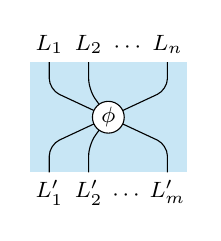
\begin{tikzpicture}[xscale=0.25,yscale=0.35]
        \footnotesize
        \fill[color=ACMBlue!20] (-4,+2) rectangle (+4,-2);
        \begin{scope}[rounded corners]
          % Input wires
          \draw (-3,+2) node[above] {$L_1$} -- (-3,+1) -- (0,0);
          \draw (-1,+2) node[above] (L2) {$L_2$} -- (-1,+1) -- (0,0);
          \draw (+3,+2) node[above] (Ln) {$L_n$} -- (+3,+1) -- (0,0);
          \path (L2) -- node[yshift=-1pt] {$\cdots$} (Ln);
          % Output wires
          \draw (-3,-2) node[below] {$L_1'$} -- (-3,-1) -- (0,0);
          \draw (-1,-2) node[below] (M2) {$L_2'$} -- (-1,-1) -- (0,0);
          \draw (+3,-2) node[below] (Mm) {$L_m'$} -- (+3,-1) -- (0,0);
          \path (M2) -- node[yshift=-1pt] {$\cdots$} (Mm);
        \end{scope}
        \node[circle,draw,fill=white,inner sep=1pt] {$\phi$};
      \end{tikzpicture}
  \]
  \pause
  Our previous example is represented as:
  \vspace{-1ex}
  \[
      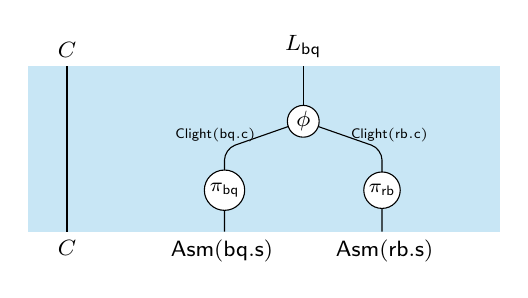
\begin{tikzpicture}[yscale=0.35]
        \footnotesize
        \fill[color=ACMBlue!20] (-3.5,+2) rectangle (+2.5,-4);
        \begin{scope}[rounded corners]
          \draw (-3,+2) node[above] {$C$}
             -- (-3,-4) node[below] {$C$};
          \draw (0,2) node[above] {$L_\kw{bq}$} -- (0,0);
          \draw (0,0) -- node[left] {\tiny $\kw{Clight}(\kw{bq.c})$} (-1,-1)
                      -- (-1,-4) node[below] {$\kw{Asm}(\kw{bq.s})\:$};
          \draw (0,0) -- node[right] {\tiny $\kw{Clight}(\kw{rb.c})$} (+1,-1)
                      -- (+1,-4) node[below] {$\:\kw{Asm}(\kw{rb.s})$};
        \end{scope}
        \begin{scope}[every node/.style={inner sep=1pt,circle,draw,fill=white,inner sep=1pt}]
          \node at (0,0) {$\phi$};
          \node at (-1,-2.5) {\scriptsize $\pi_\kw{bq}$};
          \node at (+1,-2.5) {\scriptsize $\pi_\kw{rb}$};
        \end{scope}
      \end{tikzpicture}
  \]
\end{frame}
%}}}

\begin{frame}{Issues with Compositional CompCert} %{{{
  Compositional CompCert was a remarkable achievement \\
  but it underscores the difficulty of using compositional semantics.
  \begin{itemize}
  \item
  Previously internal details become observable, \\
  so simulation relations are much more constrained.
  \item
  As a result,
  many proofs had to be redone \\
  and became much more complex.
  \end{itemize}

  \pause\vfill
  CompCertO addresses this
  by dealing with each language and pass \\
  \emph{on its own terms}:
  \begin{itemize}
    \item Languages can use their own questions and answers
    \item Calling conventions are modeled explicitly
  \end{itemize}
\end{frame}
%}}}

\section{A Double Category of Transition Systems}

\begin{frame}{Horizontal Morphisms} %{{{
  \only<1>{
    Recall the transition systems
    $L = \langle S, {\rightarrow}, I, X, Y, F \rangle \in \mathbf{TS}$
    used in CompComp:
    \begin{align*}
      I &\:\subseteq\: (\mathsf{ident} \times \mathsf{val}^* \times \mathsf{mem}) \times S
      &
      F &\:\subseteq\: S \times (\mathsf{val} \times \mathsf{mem})
      \\
      X &\:\subseteq\: S \times (\mathsf{ident} \times \mathsf{val}^* \times \mathsf{mem})
      &
      Y^{s} &\:\subseteq\: (\mathsf{val} \times \mathsf{mem}) \times S
    \end{align*}
    The questions and answers are hardcoded to correspond to C calls.
  }
  \pause
  \only<2->{
  In CompCertO, we generalize
  $L = \langle S, {\rightarrow}, I, X, Y, F \rangle : A \twoheadrightarrow B$
  to:
  \begin{align*}
    I &\:\subseteq\: B^\circ \times S
    &
    F &\:\subseteq\: S \times B^\bullet
    \\
    X &\:\subseteq\: S \times A^\circ
    &
    Y^{s} &\:\subseteq\: A^\bullet \times S
  \end{align*}
  for the \emph{language interfaces} $A = \langle A^\circ, A^\bullet \rangle$
  and $B = \langle B^\que, B^\ans \rangle$.
  }
  \pause\vfill
%  \begin{center}
%    \begin{tabular}{lccc}
%      \toprule
%      \multicolumn{4}{c}{\textbf{CompCertO} (so far)} \\
%      \midrule
%      Object & Dimension & \multicolumn{2}{c}{Ops} \\
%      \midrule
%      \textbf{Language interface} & 0 & \\
%      Transition system & 1 & & $\oplus$ \\
%      Simulation & 2 & $\mathbin;$ & $\oplus$ \\
%      \bottomrule
%    \end{tabular}
%  \end{center}
  For our purposes,
  we use the following notion of composition $L_1 \odot L_2$:
  \[
    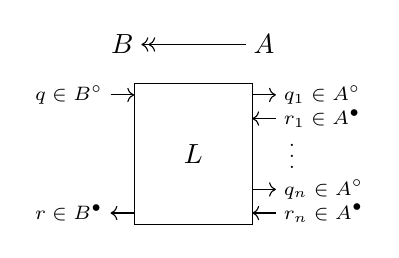
\begin{tikzpicture}[yscale=0.15,xscale=0.30]
      \draw (0,-1) rectangle (5,11) node[midway] {$L$};
      \scriptsize
      \draw[->] (-1,10) node[left] {$q \in B^\que$} -- (0,10)
          node[above=1.5em,midway] (B) {\normalsize $B$};
        \draw[->] (5,10) -- (6,10) node[right] {$q_1 \in A^\que$}
          node[above=1.5em,midway] (A) {\normalsize $A$};
        \draw[->] (6,8) node[right] {$r_1 \in A^\ans$} -- (5,8) ;
        \node[right] at (6,5.5) {$\:\vdots$};
        \draw[->] (5,2) -- (6,2) node[right] {$q_n \in A^\que$};
        \draw[->] (6,0) node[right] {$r_n \in A^\ans$} -- (5,0);
      \draw[->] (0,0) -- (-1,0) node[left] {$r \in B^\ans$};
      \draw[->>] (A) -- (B);
    \end{tikzpicture}
    \qquad
    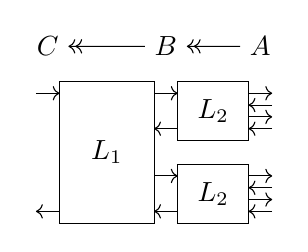
\begin{tikzpicture}[yscale=0.15,xscale=0.30]
      \draw (0,-1) rectangle (4,11) node[midway] {$L_1$};
      \draw (5,6) rectangle (8,11) node[midway] {$L_2$};
      \draw (5,-1) rectangle (8,4) node[midway] {$L_2$};
      \draw[->] (-1,10) -- (0,10) node[above=1em,midway] (C) {$C$};
        \draw[->] (4,10) -- (5,10) node[above=1em,midway] (B) {$B$};
          \draw[->] (8,10) -- (9,10) node[above=1em,midway] (A) {$A$};
          \draw[->] (9,9) -- (8,9);
          \draw[->] (8,8) -- (9,8);
          \draw[->] (9,7) -- (8,7);
        \draw[->] (5,7) -- (4,7);
        \draw[->] (4,3) -- (5,3);
          \draw[->] (8,3) -- (9,3);
          \draw[->] (9,2) -- (8,2);
          \draw[->] (8,1) -- (9,1);
          \draw[->] (9,0) -- (8,0);
        \draw[->] (5,0) -- (4,0);
      \draw[->] (0,0) -- (-1,0);
      \draw[->>] (A) -- (B);
      \draw[->>] (B) -- (C);
    \end{tikzpicture}
%    \quad
%    \begin{tikzpicture}[yscale=0.15,xscale=0.30]
%      \draw (5,-1) rectangle (8,4) node[midway] {$\kw{id}_A$};
%      \draw[->] (4,3) node[left] {$q \in A^\que$} -- (5,3) node[above=2em,midway] (A2) {$A$};
%        \draw[->] (8,3) -- (9,3) node[above=2em,midway] (A1) {$A$} node[right] {$q$};
%        \draw[->] (9,0) node[right] {$r \in A^\ans$} -- (8,0);
%      \draw[->] (5,0) -- (4,0) node[left] {$r$};
%      \draw[->>] (A1) -- (A2);
%    \end{tikzpicture}
  \]
%  Fortunately, $\odot$ is an under-approximation of $\oplus$:
%  \[
%    \kw{Asm}(M_1) \odot \kw{Asm}(M_2) \le
%    \kw{Asm}(M_1) \oplus \kw{Asm}(M_2)
%  \]
\end{frame}
%}}}

\begin{frame}[fragile]{Vertical Morphisms} %{{{
  To connect source and target languages such as
  \[
    \mathsf{Clight}(p) : \mathcal{C} \twoheadrightarrow \mathcal{C}
    \qquad
    \textit{vs}
    \qquad
    \mathsf{Asm}(p') : \mathcal{A} \twoheadrightarrow \mathcal{A}
    \,,
  \]
  CompCertO introduces \emph{simulation conventions}
  $\mathbb{R} : \mathcal{C} \leftrightarrow \mathcal{A}$,
  which parameterize \\
  the relationship between source- and target-level interactions:
  \[
    \begin{tikzcd}
      \mathcal{C}^\circ \ni {} \hspace{-3em} &
      q_1 \ar[r, dash, "I_1"] \ar[d, "\mathbb{R}^\circ"', dash] & s_1 \ar[d, "\rho", dash, dashed] &
      s_1 \ar[r] \ar[d, dash, "\rho"'] & s_1' \ar[d, dashed, dash, "\rho"] &
      s_1 \ar[r, dash, "F_1"] \ar[d, dash, "\rho"'] & r_1 \ar[d, "\mathbb{R}^\bullet", dashed, dash]
      & \hspace{-3em} {} \in \mathcal{C}^\bullet
      \\
      \mathcal{A}^\circ \ni {} \hspace{-3em} &
      q_2 \ar[r, dash, dashed, "I_2"'] & s_2 &
      s_2 \ar[r, dashed] & s_2' & s_2 \ar[r, dashed, dash, "F_2"] & r_2
      & \hspace{-3em} {} \in \mathcal{A}^\bullet
    \end{tikzcd}
  \]
  Simulation conventions compose vertically as $\mathbb{R}_1 \mathbin; \mathbb{R}_2$.
\end{frame}
%}}}

\begin{frame}[fragile]{Simulations} %{{{
  Simulations now have two-dimentional types and compose in both directions:
\[
  \pi : L_1 \le_{\mathbf{R}_A \twoheadrightarrow \mathbf{R}_B} L_2
  \qquad
  \qquad
  \begin{tikzcd}
    A_1 \ar[d, leftrightarrow, "\mathbf{R}_A"']
        \ar[r, twoheadrightarrow, "L_1"] &
    B_1 \ar[d, leftrightarrow, "\mathbf{R}_B"] \\
    A_2 \ar[r, twoheadrightarrow, "L_2"'] &
    B_2
  \end{tikzcd}
\]

  \pause
  \begin{center}
    \begin{tabular}{llcll}
      \toprule
      \multicolumn{5}{c}{\textbf{CompCertO}} \\
      \midrule
      Object & & Dimension & \multicolumn{2}{c}{Ops} \\
      \midrule
      Language interface & $A$ & 0 & \\
      Transition system & $L : A \twoheadrightarrow B$ & 1 & & $\odot$ \\
      Simulation convention & $\mathbb{R} : A \leftrightarrow B$ & 1 & $\mathbin;$ \\
      Simulation & $\rho : L_1 \le_\mathbb{R \twoheadrightarrow S} L_2$ & 2 & $\mathbin;$ & $\odot$ \\
      \bottomrule
    \end{tabular}
  \end{center}
\end{frame}
%}}}

\begin{frame}[fragile]{CompCertO in Pasting Diagrams} %{{{
\[
  \begin{tikzcd}
    {}
      \only<2>{\bullet}
      \only<3>{\mathcal{C}}
      \only<2>{\ar[rrrr, "L_\kw{bq}", dash]}
      \only<3>{\ar[rrrr, twoheadleftarrow, "L_\kw{bq}"]}
      \only<2-3>{\ar[dd, Rightarrow, dash]}
      &&
    {}
      \only<1>{L_1}
      \only<1>{\ar[dd, Rightarrow, "\phi"]}
      &&
    {}
      \only<2>{\bullet}
      \only<3>{\top}
      \only<2>{\ar[dd, Rightarrow, dash]}
      \only<3>{\ar[dd, leftrightarrow, "\varnothing"]}
  \\
    && \only<2-3>{\phi}
  \\
    {}
      \only<2>{\bullet}
      \only<3>{\mathcal{C}}
      \only<2>{\ar[rr, "\kw{Clight}(\kw{bq.c})", dash]}
      \only<3>{\ar[rr, "\kw{Clight}(\kw{bq.c})", twoheadleftarrow]}
      \only<2>{\ar[dd, Rightarrow, dash]}
      \only<3>{\ar[dd, leftrightarrow, "\mathbb{C}"]}
      &&
    {}
      \only<1>{L_2}
      \only<1>{\ar[dd, Rightarrow, "\pi"]}
      \only<2>{\bullet}
      \only<3>{\mathcal{C}}
      \only<2-3>{\ar[rr, "\kw{Clight}(\kw{rb.c})", twoheadleftarrow]}
      \only<2>{\ar[dd, Rightarrow, dash]}
      \only<3>{\ar[dd, leftrightarrow, "\mathbb{C}"]}
      &&
    {}
      \only<2>{\bullet}
      \only<3>{\mathcal{C}}
      \only<2>{\ar[dd, Rightarrow, dash]}
      \only<3>{\ar[dd, leftrightarrow, "\mathbb{C}"]}
  \\
    & \only<2->{\pi_\kw{bq}} &
    & \only<2->{\pi_\kw{rb}} &
  \\
    {} 
      \only<2>{\bullet}
      \only<3>{\mathcal{A}}
      \only<2->{\ar[rr, "\kw{Asm}(\kw{bq.s})", twoheadleftarrow]}
      &&
    {}
      \only<1>{L_3}
      \only<2>{\bullet}
      \only<3>{\mathcal{A}}
      \only<2->{\ar[rr, "\kw{Asm}(\kw{rb.s})", twoheadleftarrow]}
      &&
    {}
      \only<2>{\bullet}
      \only<3>{\mathcal{A}}
  \end{tikzcd}
\]
\end{frame}
%}}}

\begin{frame}[fragile]{CompCertO in String Diagrams} %{{{
A simulation
\[
  \phi : L_1 \odot \cdots \odot L_n
  \le_{\mathbb{R}_1 \mathbin; \cdots \mathbin; \mathbb{R}_k
     \twoheadrightarrow
     \mathbb{S}_1 \mathbin; \cdots \mathbin; \mathbb{S}_l}
  L_1' \odot \cdots \odot L_m'
\]
can be represented as:
\[
  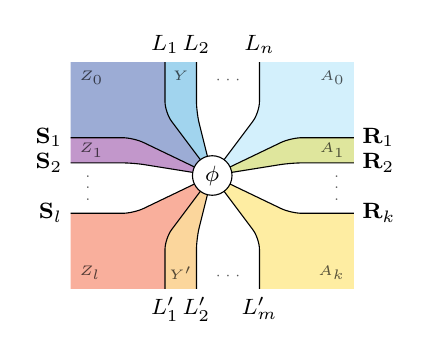
\begin{tikzpicture}[xscale=0.2,yscale=0.16]
    \footnotesize

    % Coordinates
    \path (0,0) coordinate (C)
      (-3,+5) coordinate (L1c) +(0,+4) coordinate (L1)
      (-1,+5) coordinate (L2c) +(0,+4) coordinate (L2)
      (+3,+5) coordinate (Lnc) +(0,+4) coordinate (Ln)
      (+5, 3) coordinate (S1c) +(+4,0) coordinate (S1)
      (+5, 1) coordinate (S2c) +(+4,0) coordinate (S2)
      (+5,-3) coordinate (Snc) +(+4,0) coordinate (Sn)
      (-3,-5) coordinate (M1c) +(0,-4) coordinate (M1)
      (-1,-5) coordinate (M2c) +(0,-4) coordinate (M2)
      (+3,-5) coordinate (Mnc) +(0,-4) coordinate (Mn)
      (-5, 3) coordinate (R1c) +(-4,0) coordinate (R1)
      (-5, 1) coordinate (R2c) +(-4,0) coordinate (R2)
      (-5,-3) coordinate (Rnc) +(-4,0) coordinate (Rn)
      ;

    % Background regions
    \fill[ACMBlue\filltint] (C)
      [rounded corners] -- (L1c)
      [sharp corners] -- (L1) -- (L2)
      [rounded corners] -- (L2c)
      [sharp corners] -- cycle;
    \fill[ACMLightBlue\filltint] (C)
      [rounded corners] -- (Lnc)
      [sharp corners] -- (Ln) -| (S1)
      [rounded corners] -- (S1c)
      [sharp corners] -- cycle;
    \fill[ACMGreen\filltint] (C)
      [rounded corners] -- (S2c)
      [sharp corners] -- (S2) -- (S1)
      [rounded corners] -- (S1c)
      [sharp corners] -- cycle;
    \fill[ACMYellow\filltint] (C)
      [rounded corners] -- (Mnc)
      [sharp corners] -- (Mn) -| (Sn)
      [rounded corners] -- (Snc)
      [sharp corners] -- cycle;
    \fill[ACMOrange\filltint] (C)
      [rounded corners] -- (M1c)
      [sharp corners] -- (M1) -- (M2)
      [rounded corners] -- (M2c)
      [sharp corners] -- cycle;
    \fill[ACMRed\filltint] (C)
      [rounded corners] -- (M1c)
      [sharp corners] -- (M1) -| (Rn)
      [rounded corners] -- (Rnc)
      [sharp corners] -- cycle;
    \fill[ACMPurple\filltint] (C)
      [rounded corners] -- (R2c)
      [sharp corners] -- (R2) -- (R1)
      [rounded corners] -- (R1c)
      [sharp corners] -- cycle;
    \fill[ACMDarkBlue\filltint] (C)
      [rounded corners] -- (L1c)
      [sharp corners] -- (L1) -| (R1)
      [rounded corners] -- (R1c)
      [sharp corners] -- cycle;

    % Region labels
    \begin{scope}[opacity=0.66,outer sep=1pt]
      \tiny

      % Language interfaces
      \path (R1) |- node[below right] {$Z_0$} (L1);
      \path (R1) -- node[right] {$Z_1$} (R2);
      \path (Rn) |- node[above right] {$Z_l$} (M1);
      \path (M1) -- node[above] {$Y'$} (M2);
      \path (Mn) -| node[above left] {$A_k$} (Sn);
      \path (L1) -- node[below] {$Y$} (L2);
      \path (Ln) -| node[below left] {$A_0$} (S1);
      \path (S1) -- node[left] {$A_1$} (S2);

      % Dot dot
      \path (L2) -- node[below,yshift=-2pt] {$\cdots$} (Ln);
      \path (S2) -- node[left,yshift=3pt,xshift=-2pt] {$\vdots$} (Sn);
      \path (M2) -- node[above] {$\cdots$} (Mn);
      \path (R2) -- node[right,yshift=3pt,xshift=2pt]  {$\vdots$} (Rn);
    \end{scope}

    % Strings
    \begin{scope}
      \draw (C)
        [rounded corners] -- (L1c)
        [sharp corners] -- (L1) node[above] {$L_1$};
      \draw (L2) node[above] {$L_2$}
        [rounded corners] -- (L2c)
        [sharp corners] -- (C);
      \draw (C)
        [rounded corners] -- (Lnc)
        [sharp corners] -- (Ln) node[above] {$L_n$};
      \draw (C)
        [rounded corners] -- (Mnc)
        [sharp corners] -- (Mn) node[below] {$L'_m$};
      \draw (M2) node[below] {$L'_2$}
        [rounded corners] -- (M2c)
        [sharp corners] -- (C);
      \draw (C)
        [rounded corners] -- (M1c)
        [sharp corners] -- (M1) node[below] {$L'_1$};
    \end{scope}
    \begin{scope}%[thick]
      \draw (S1) node[right] {$\mathbf{R}_1$}
        [rounded corners] -- (S1c)
        [sharp corners] -- (C);
      \draw (C)
        [rounded corners] -- (S2c)
        [sharp corners] -- (S2) node[right] {$\mathbf{R}_2$};
      \draw (Sn) node[right] {$\mathbf{R}_k$}
        [rounded corners] -- (Snc)
        [sharp corners] -- (C);
      \draw (R1) node[left] {$\mathbf{S}_1$}
        [rounded corners] -- (R1c)
        [sharp corners] -- (C);
      \draw (C)
        [rounded corners] -- (R2c)
        [sharp corners] -- (R2) node[left] {$\mathbf{S}_2$};
      \draw (Rn) node[left] {$\mathbf{S}_l$}
        [rounded corners] -- (Rnc)
        [sharp corners] -- (C);
    \end{scope}

    % Node
    \node[draw,fill=white,circle,inner sep=2pt] at (C) {$\phi$};

  \end{tikzpicture}
\]
\end{frame}

\begin{frame}{CompCertO in String Diagrams (example)}
\[
  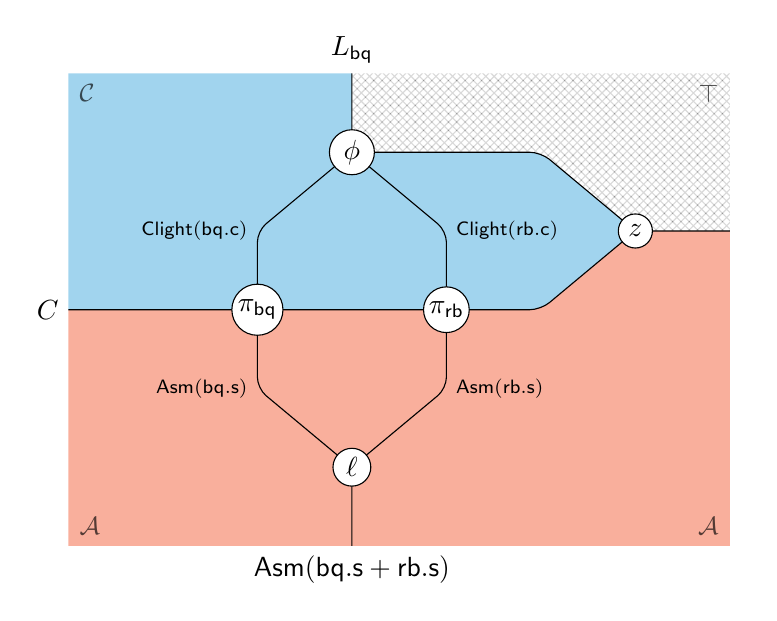
\begin{tikzpicture}[xscale=1.2]

    % Background regions
    \fill[ACMBlue\filltint]
      (-3, 0)
      [rounded corners] -- (2,0)
      [sharp corners] -- (3,1)
      [rounded corners] -- (2,2)
      [sharp corners] -- (0,2) -- (0,3) -| cycle;
    \fill[ACMRed\filltint]
      (-3, 0)
      [rounded corners] -- (2,0)
      [sharp corners] -- (3,1) -- (4,1) -- (4,-3) -| cycle;
    \fill[pattern=crosshatch,opacity=0.15]
      (4,1) -- (3,1)
      [rounded corners] -- (2,2)
      [sharp corners] -| (0,3) -| cycle;

    % Region labels
    \begin{scope}[opacity=0.66,outer sep=1pt]
      \small
      \node[below right] at (-3,3) {$\mathcal{C}$};
      \node[below left] at (4,3) {$\top$};
      \node[above right] at (-3,-3) {$\mathcal{A}$};
      \node[above left] at (4,-3) {$\mathcal{A}$};
    \end{scope}

    % Strings
    \begin{scope}
      % Transition systems
      \draw (0,3) node[above] {$L_\kw{bq}$}
         -- (0,2)
         [rounded corners]
         -- (-1, 1) node[left] {\scriptsize $\kw{Clight}(\kw{bq.c})$}
         -- (-1,-1) node[left] {\scriptsize $\kw{Asm}(\kw{bq.s})$}
         [sharp corners]
         -- (0,-2)
         -- (0,-3) node[below] {$\kw{Asm}(\kw{bq.s} + \kw{rb.s})$};
      \draw (0,2)
         [rounded corners]
         -- (1, 1) node[right] {\scriptsize $\kw{Clight}(\kw{rb.c})$}
         -- (1,-1) node[right] {\scriptsize $\kw{Asm}(\kw{rb.s})$}
         [sharp corners]
         -- (0,-2);
      % Simulation conventions
      \draw (-3,0) node[left] {$\mathbb{C}$}
         [rounded corners] -- (2,0)
         [sharp corners] -- (3,1) -- (4,1) node[right] {$\varnothing$};
      \draw (0,2)
         [rounded corners] -- node[above] {\small $\varnothing$} (2,2)
         [sharp corners] -- (3,1);
    \end{scope}

    % Nodes
    \begin{scope}[every node/.style={draw,fill=white,circle,inner sep=2pt}]
       \node at (0,2) {$\phi$};
       \node[inner sep=1pt] at (-1,0) {$\pi_\kw{bq}$};
       \node[inner sep=1pt] at (+1,0) {$\pi_\kw{rb}$};
       \node at (0,-2) {$\ell$};
       \node at (3,1) {$z$};
    \end{scope}
  \end{tikzpicture}
\]
\end{frame}
%}}}

\section{Abstract State and Spatial Composition}

\begin{frame}[fragile]{Abstract Specifications} %{{{
  What would be a good specification for our example:

  \vspace{1ex}
  \begin{columns}
    \scriptsize
    \begin{column}{0.45\textwidth}
\textbf{rb.c}
\begin{minted}{C}
/* Encapsulated state */
static int c1, c2;
static V buf[N];

/* Accessors */
int inc1() { int i = c1++; c1 %= N; return i; }
int inc2() { int i = c2++; c2 %= N; return i; }
V get(int i) { return buf[i]; }
void set(int i, V val) { buf[i] = val; }
\end{minted}
    \end{column}
    \begin{column}{0.45\textwidth}
\textbf{bq.c}
\begin{minted}{C}
/* Underlay signature */
extern int inc1(void);
extern int inc2(void);
extern V get(int i);
extern void set(int i, V val);

/* Layer implementation */
void enq(V val) { set(inc2(), val); }
V deq() { return get(inc1()); }
\end{minted}
    \end{column}
  \end{columns}

  \vfill
  As a user,
  we would prefer not to deal with low-level details about the memory,
  and rely instead on an abstract description:
\[
  %\Gamma_\kw{bq} : \top \twoheadrightarrow \mathcal{C} \mathbin@ D_\kw{bq}
  %\qquad
  %\text{such that}
  %\qquad
  \begin{array}{l}
    \Gamma_\kw{bq} \:\vDash\:
      \kw{enq}(v) @ \vec{q}
      \:\rightarrowtail\:
      {*} @ \vec{q}v
    \\
    \Gamma_\kw{bq} \:\vDash\:
      \kw{deq}() @ v\vec{q}
      \:\rightarrowtail\:
      v @ \vec{q}
  \end{array}
  \quad \text{where} \quad
  \vec{q} \in D_\kw{bq} := \kw{val}^*
\]
\end{frame}
%}}}

\begin{frame}{Abstract Specifications} %{{{
Likewise,
to prove the implementation correct,
we may want to rely on
\begin{align*}
  \Gamma_\kw{rb} &\vDash
    \kw{get}(i)@(b, c_1, c_2) \rightarrowtail
    b_i@(b, c_1, c_2) \\
  \Gamma_\kw{rb} &\vDash
    \kw{set}(i, v)@(b, c_1, c_2) \rightarrowtail
    *@(b[i := v], c_1, c_2) \\
  \Gamma_\kw{rb} &\vDash
    \kw{inc1}()@(b, c_1, c_2) \rightarrowtail
    c_1@(b, c_1\!\!+\!\!1, c_2) \\
  \Gamma_\kw{rb} &\vDash
    \kw{inc2}()@(b, c_1, c_2) \rightarrowtail
    c_2@(b, c_1, c_2\!\!+\!\!1)
\end{align*}
which specifies $\kw{rb.c}$ in terms of
$D_\kw{rb} := V^N \times \mathbb{N} \times \mathbb{N}$

\vfill\pause
%This is the principle behind \emph{certified abstraction layers}.

CompCertO's language interfaces and simulation conventions can help us do this! \\
But it requires a good way to deal with abstract state.
\end{frame}
%}}}

\begin{frame}{Adjoining state to language interfaces} %{{{
Consider the following construction on language interfaces:
\[
  A \mathbin@ U := \langle A^\que \times U, \, A^\ans \times U \rangle
\]
That is, we extend $A$ with a state component taken in the set $U$.

\vfill \pause
The language interface used for C semantics can be described as:
\[
  \kw{Clight}(M) : \mathcal{C} \mathbin@ \kw{mem} \twoheadrightarrow
      \mathcal{C} \mathbin@ \kw{mem}
  \qquad \text{where} \quad
  \mathcal{C} = \langle \kw{ident} \times \kw{val}^*, \, \kw{val} \rangle
\]
\pause
The abstract specifications are typed as:
\[
  \begin{array}{c}
    \Gamma_\kw{bq} : \top \twoheadrightarrow \mathcal{C} \mathbin@ D_\kw{bq} \\
    \Gamma_\kw{rb} : \top \twoheadrightarrow \mathcal{C} \mathbin@ D_\kw{rb}
  \end{array}
  \qquad \text{where} \quad
  \top = \langle \varnothing, \varnothing \rangle
\]
But how can we interface client code with abstract specifications?
\end{frame}
%}}}

\begin{frame}[fragile]{Spatial compositionality} %{{{
  We turn $@$ into yet another dimension of compositionality:
  \begin{itemize}
    \item Transition systems combine with a \emph{lens} $f : U \leftrightarrows V$
    \item Simulation conventions easily combine with a relation $R \subseteq U \times V$
    \item Simulations can be extended in a similar way.
  \end{itemize}

  As before, we can use string diagrams to combine two kinds of composition. \\
  For example, to interface $\kw{bq.c}$ with $\Gamma_\kw{rb}$:
\[
  \begin{array}{r@{}l}
    L_\kw{bq} :=
    (\kw{Clight}(\kw{bq.c}) \mathbin@ D_\kw{rb}) &{} \odot {} \\
    (\mathcal{C} \mathbin@ \langle \kw{mem} ] \mathbin@ D_\kw{rb}) &{} \odot
    \Gamma_\kw{rb} \: = \:
  \end{array}
  {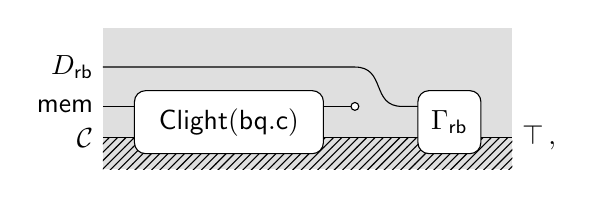
\begin{tikzpicture}[xscale=0.4,yscale=0.2,baseline=6mm]
    % Background
    \fill[tssdbg]
      (1,-2) rectangle (14,7);
    \fill[pattern=north east lines]
      (1,-2) rectangle (14,0);
    % Wires
    \draw (1,0) node[left] {$\mathcal{C}$}
      -- (14,0) node[right] {$\top\,,$};
    %\draw (0,2) node[left] {$\kw{mem}$}
    %  -- (9,2) .. controls +(1,0) and +(-1,0) .. (11,5)
    %  -- (13,5)
    %    node[circle,inner sep=1pt,draw,fill=white] {}
    %    node[right] {$\kw{mem}$};
    \draw (1,2) node[left] (mem) {$\kw{mem}$}
      -- (9,2) node[circle,inner sep=1pt,draw,fill=white] {};
    \draw (1,4.5) node[left] {$D_\kw{rb}$}
      -- (9,4.5) .. controls +(1,0) and +(-1,0) .. (10.5,2)
      -- (11,2);
    %\node[above,inner sep=1pt] at (10,0)
    %  {\footnotesize $\mathcal{C}$};
    % Boxes
    \draw[fill=white,rounded corners]
      ( 2,-1) rectangle ( 8,3) node[midway] {$\kw{Clight}(\kw{bq.c})$}
      (11,-1) rectangle (13,3) node[midway] {$\Gamma_\kw{rb}$};
  \end{tikzpicture}}
\]
where $\langle \kw{mem} ]$ is a trivial lens which ``bounces'' the memory state unchanged.
\end{frame}
%}}}

\begin{frame}{Concretizing state}
  Consider $\Gamma_\kw{rb} : \top \twoheadrightarrow \mathcal{C} \mathbin@ D_\kw{rb}$
  vs.~its implementation $\kw{rb.c}$ in terms of $\mathcal{C} \mathbin@ \kw{mem}$. \\
  The corresponding correctness property can be expressed as:
  \[
    \Gamma_\kw{rb} : \varnothing \twoheadrightarrow \mathcal{C} \mathbin@ R_\kw{rb}
    \qquad \qquad
    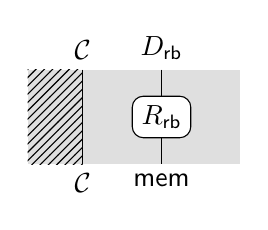
\begin{tikzpicture}[xscale=1,yscale=0.6,baseline=(R.base)]
      \fill[scsdbg] (0.3,0) rectangle (3,2);
      \fill[pattern=north east lines] (0.3,0) rectangle (1,2);
      \draw (1,2) node[above] {$\mathcal{C}$}
        -- (1,0) node[below] {$\mathcal{C}$};
      \draw (2,2) node[above] {$D_\kw{rb}$}
        -- (2,1) node[rounded corners,draw,fill=white] (R) {$R_\kw{rb}$}
        -- (2,0) node[below] {$\kw{mem}$};
    \end{tikzpicture}
  \]
  where $R_\kw{rb} \subseteq D_\kw{rb} \times \kw{mem}$ explains how abstract data
  is implemented.
\end{frame}

\begin{frame}{Summary of the framework} %{{{
  \begin{center}
  \footnotesize
  \begin{tabular}{
    lllc
    c@{\:\:\:}c@{\:\,}c@{\:}c@{}c
    c@{\hspace{1em}}c@{\:\,}c@{}c
  }
    \toprule
    & Role & Components & Notation &
      \multicolumn{5}{c}{Compose} & \multicolumn{4}{c}{Diagrams} \\
    & & & && H & V & S &&& $\mathbb{H}$ & $\mathbb{V}$
    \\
    \midrule
    Active &
      Interface
        & Language interfaces & $A, B, C$ && & & $\mathbin@$
    \\ &
      Behavior
        & Transition systems & $L : A \twoheadrightarrow B \in \mathbf{TS}$ &&
            $\odot$ & & $\mathbin@$ &&& $\odot$ & $\mathbin@$
    \\ &
      Abstraction
        & Simulation conventions & $\mathbf{R} : A \leftrightarrow B \in \mathbf{SC}$ &&
            & $\mathbin;\,$ & $\mathbin@$ &&& $\mathbin@$ & $\,\mathbin;$
    \\ &
      Refinement
        & Simulations &
          $\hspace{-2em} \pi :
           L^\sharp \le_{\mathbf{R} \twoheadrightarrow \mathbf{S}} L^\flat \in \mathbf{TSC}$ &&
          $\odot$ & $\mathbin;\,$ & $\mathbin@$ &&& $\odot$ & $\,\mathbin;$
    \\
    \midrule
    Passive &
      Interface
        & Sets & $U, V$ && & & $\times$ \\ &
      Behavior
        & Lenses & $f : U \lensarrow V \in \mathbf{Lens}$ &&
            $\circ$ & & $\times$ &&& $\circ$ & $\times$ \\ &
      Abstraction
        & Simulation relations & $R \subseteq U \times V \in \mathbf{Rel}$ &&
            & $\mathbin;$ & $\times$ &&& $\times$ & $\,\mathbin;\,$ \\ &
      Refinement
        & Bisimulations &
          $\hspace{-1.5em} \phi : f \lensle_{R \lensarrow S} g \in \mathbf{LSR}$ &&
          $\circ$ & $\mathbin;$ & $\times$ &&& $\circ$ & $\,\mathbin;\,$ \\
    \bottomrule
  \end{tabular}
  \end{center}
\end{frame}
%}}}

\begin{frame}{Compositional state vs. CompCert memory}
  To preserve compositionality when concretizing abstract state, \\
  we can use separation algebra as
  a relation ${\bullet} \subseteq (\kw{mem} \times \kw{mem}) \times \kw{mem}$:
  \[
    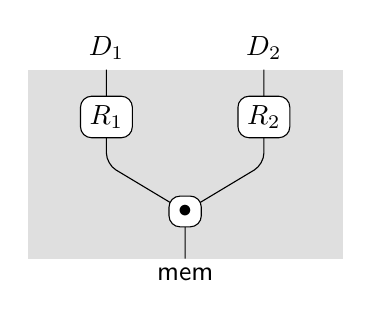
\begin{tikzpicture}[xscale=1,yscale=0.6,baseline=(R.base)]
      \fill[scsdbg] (0,-2) rectangle (4,2);
      \draw (1,2) node[above] {$D_1$}
        -- (1,1) node[rounded corners,draw,fill=white] (R) {$R_1$}
        [rounded corners] -- (1,0)
        [sharp corners] -- (2,-1)
        -- (2,-2) node[below] {$\kw{mem}$};
      \draw (3,2) node[above] {$D_2$}
        -- (3,1) node[rounded corners,draw,fill=white] (R) {$R_2$}
        [rounded corners] -- (3,0)
        [sharp corners] -- (2,-1) node[draw,fill=white,rounded corners] {$\bullet$};
    \end{tikzpicture}
  \]
  \pause
  Properties of interest can be expressed as simulations, for example
  \begin{itemize}
    \item $\kw{id}_{\kw{mem} \times \kw{mem} \times \kw{mem}}
      \equiv_{({\bullet} \mathbin@ \kw{mem}) \mathbin; {\bullet}
          \twoheadrightarrow
         (\kw{mem} \mathbin@ {\bullet}) \mathbin;  \bullet}
       \kw{id}_\kw{mem}$
    \pause
    \item $\kw{Clight}(M) \mathbin@ \kw{mem}
       \le_{\mathcal{C} \mathbin@ {\bullet} \twoheadrightarrow
            \mathcal{C} \mathbin@ {\bullet}}
    \kw{Clight}(M)$
  \end{itemize}
\end{frame}
  
\begin{frame}{Three dimenstions of compositionality}
  Simulation string diagrams can also incorporate $@$ as \emph{depth}.
  \[
  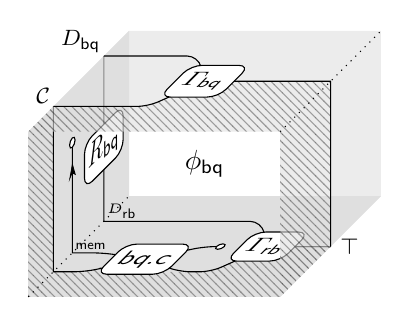
\begin{tikzpicture}[sdp]

    %% Left and bottom faces

    % Background area
    \fill[tssdbg] (0,0,0) -- (0,6,0) -- (0,6,8)
               -- (0,0,8) -- (8,0,8) -- (8,0,0) -- cycle;
    \draw[thin,dotted] (0,0,0) -- (0,0,8);
    \fill[act] (0,0,0) -- (0,6,0)
      -- (0,6,2) -- (0,0,2)
      [rounded corners] -- (1,0,2)
      [sharp corners] -- (2,0,3)
      [rounded corners] -- (3,0,2) -- (5,0,2)
      [sharp corners] -- (6,0,4) -- (8,0,4)
      -- (8,0,0) -- cycle;

    % Strings
    \draw (0,6,2) -- (0,0,2)
      [rounded corners] -- (1,0,2)
      [sharp corners] -- (2.5,0,3)
      [rounded corners] -- (4,0,2) -- (5,0,2)
      [sharp corners] -- (6,0,4)
      -- (8,0,4) node[right] {\footnotesize $\top$};
    \draw (0,4,3.5)
      node[scn,bln] {}
      -- (0,3,3.5) \companion
      -- (0,0,3.5)
      node[above right,inner sep=1pt] {\tiny $\kw{mem}$}
      [rounded corners] -- (1,0,3.5)
      [sharp corners] -- (2.5,0,3)
      node[tsn] {$\kw{bq.c}$}
      [rounded corners] -- (4,0,4)
      [sharp corners] -- (4.5,0,4)
      node[tsn,bln] {};
    \draw (0,6,6)
      -- (0,2.7,6)
      node[scn] {$R_\kw{bq}$}
      -- (0,0,6)
      node[above right,inner sep=1pt] {\tiny $D_\kw{rb}$}
      [rounded corners] -- (5,0,6)
      [sharp corners] -- (6,0,4)
      node[tsn] (rb) {$\Gamma_\kw{rb}$}
      -- (8,0,4);

    %% Center label

    \node%[draw,circle,inner sep=1pt]
       at (4,3,4) {$\phi_\kw{bq}$};

    %% Top and right

    % Background
    \fill[tssdbg,opacity=0.6]
      (0,6,0) -- (8,6,0) -- (8,0,0) -- (8,0,8) -- (8,6,8) -- (0,6,8) -- cycle;
    \draw[thin,dotted] (8,6,0) -- (8,6,8);
    \fill[act]
      (0,6,0) -- (0,6,2)
      [rounded corners] -- (3,6,2)
      [sharp corners] -- (4,6,4)
      -- (8,6,4) -- (8,0,4) -- (8,0,0) -- (8,6,0) -- cycle;

    % Strings and nodes
    \draw (0,6,2) node[above left,inner sep=1pt] {\footnotesize $\mathcal{C}$}
      [rounded corners] -- (3,6,2)
      [sharp corners] -- (4,6,4)
      -- (8,6,4) -- (8,0,4);
    \draw (0,6,6) node[above left, inner sep=1pt] {\footnotesize $D_\kw{bq}$}
      [rounded corners] -- (3,6,6)
      [sharp corners] -- (4,6,4)
      node[tsn] {$\Gamma_\kw{bq}$};

  \end{tikzpicture}
  \]
  Overall, many properties of interest can be put into the form of simulation ``cubes''
  of the kind above, and proofs can be glued together geometrically.
\end{frame}

\section{Conclusion}

\begin{frame}{Conclusion}
This is joint work with
Yu Zhang, Zhong Shao and Yuting Wang. \\
We are hoping to use thi framework
for large-scale verification applications.

Some other things we did:
\begin{itemize}
  \item Model of certified abstraction layers within this framework
  \item Encapsulated state
  \item $\kw{ClightP}$ language with private variables
\end{itemize}

\vfill\pause
Last thoughts:
\begin{itemize}
  \item Compositional semantics for compilers are hard but interesting
  \item Semantics and higher category theory can be useful for engineering
\end{itemize}

Please feel free to request our paper draft from me!
(\texttt{jeremie.koenig@gmail.com})
\end{frame}

%\begin{frame}
%Sometimes there is a correspondence between
%horizontal and vertical morphisms, \\
%formalized by the notion of companions and conjoints
%in a double category:
%\[
%  \begin{array}{r@{}l}
%    \begin{tikzpicture}[scale=0.4,baseline] %{{{
%      % Background
%      \begin{scope}
%        \fill[ACMBlue!50] (1,2)
%          [rounded corners] -- (1,1)
%          [sharp corners] -- (2,1) |- cycle;
%        \fill[pattern=crosshatch dots,opacity=0.2] (0,2) -- (1,2)
%          [rounded corners] -- (1,1)
%          [sharp corners] -- (2,1) -- (2,0) -| cycle;
%      \end{scope}
%      % Region labels
%      \begin{scope}[opacity=0.5]
%        \tiny
%        %\node[above right] at (0,0) {$\mathbf{I}$};
%        %\node[below left] at (2,2) {$U$};
%      \end{scope}
%      % Strings
%      \begin{scope}
%        \footnotesize
%        \draw (1,2) node[above] {$\mathbb{R}^*$}
%          [rounded corners] -- (1,1)
%          [sharp corners] -- (2,1)
%          node[right] {$\mathbb{R}$};
%      \end{scope}
%    \end{tikzpicture}
%    %}}}
%    &
%    \begin{tikzpicture}[scale=0.4,baseline] %{{{
%      % Background
%      \begin{scope}
%        \fill[ACMBlue!50] (0,2) -- (0,1)
%          [rounded corners] -- (1,1)
%          [sharp corners] -- (1,0) -- (2,0) |- cycle;
%        \fill[pattern=crosshatch dots,opacity=0.2] (0,1)
%          [rounded corners] -- (1,1)
%          [sharp corners] -- (1,0) -| cycle;
%      \end{scope}
%      % Region labels
%      \begin{scope}[opacity=0.5]
%        \tiny
%        %\node[above right] at (0,0) {$\mathbf{I}$};
%        %\node[below left] at (2,2) {$U$};
%      \end{scope}
%      % Strings
%      \begin{scope}
%        \footnotesize
%        \draw (0,1) %node[left] {$\mathbb{R}^*$}
%          [rounded corners] -- (1,1)
%          [sharp corners] -- (1,0)
%          node[below] {$\mathbb{R}_*$};
%      \end{scope}
%    \end{tikzpicture}
%    %}}}
%    \\
%    \begin{tikzpicture}[scale=0.4,baseline] %{{{
%      % Background
%      \begin{scope}
%        \fill[ACMBlue!50] (1,0)
%          [rounded corners] -- (1,1)
%          [sharp corners] -- (2,1) |- cycle;
%        \fill[pattern=crosshatch dots,opacity=0.2] (0,0) -- (1,0)
%          [rounded corners] -- (1,1)
%          [sharp corners] -- (2,1) -- (2,2) -| cycle;
%      \end{scope}
%      % Region labels
%      \begin{scope}[opacity=0.5]
%        \tiny
%        %\node[above right] at (0,0) {$\mathbf{I}$};
%        %\node[above left] at (2,0) {$U$};
%      \end{scope}
%      % Strings
%      \begin{scope}
%        \footnotesize
%        \draw (1,0) node[below] {$\mathbb{R}^*$}
%          [rounded corners] -- (1,1)
%          [sharp corners] -- (2,1)
%          node[right] {$\mathbb{R}$};
%      \end{scope}
%    \end{tikzpicture}
%    %}}}
%    &
%    \begin{tikzpicture}[scale=0.4,baseline] %{{{
%      % Background
%      \begin{scope}
%        \fill[ACMBlue!50] (2,2) -- (1,2)
%          [rounded corners] -- (1,1)
%          [sharp corners] -- (0,1) -- (0,0) -| cycle;
%        \fill[pattern=crosshatch dots,opacity=0.2] (1,2)
%          [rounded corners] -- (1,1)
%          [sharp corners] -- (0,1) |- cycle;
%      \end{scope}
%      % Region labels
%      \begin{scope}[opacity=0.5]
%        \tiny
%        %\node[above right] at (0,0) {$\mathbf{I}$};
%        %\node[above left] at (2,0) {$U$};
%      \end{scope}
%      % Strings
%      \begin{scope}
%        \footnotesize
%        \draw (1,2) %node[above] {$\mathbb{R}$}
%          [rounded corners] -- (1,1)
%          [sharp corners] -- (0,1)
%          ; %node[left] {$\mathbb{R}_*$};
%      \end{scope}
%    \end{tikzpicture}
%    %}}}
%  \end{array}
%\]
%This could be useful to give semantics to multi-languages,
%with $\mathbb{R}^*$, $\mathbb{R}_*$ representing language boundaries.
%
%For example, the CompCertO correctness theorem could now be stated as:
%\[
%  \kw{Clight}(p) \le \mathbb{C}^* \odot \kw{Asm}(p') \odot \mathbb{C}_* :
%    \mathcal{C} \mathbin@ \kw{mem} \twoheadrightarrow
%    \mathcal{C} \mathbin@ \kw{mem}
%\]
%\end{frame}

\end{document}
